\chapter{Fundamental concepts of quantum computation and information}
\label{Chapter1}

This chapter provides a brief introduction to quantum computation and quantum information \cite{Nielsen}. Firstly,  quantum bits, or qubits, are introduced and their properties are illustrated in the state vector formalism. We also define the measurement operation, through which we infer information from a quantum state but destroy its coherence. Then, we introduce the density matrix representation of the states. 
It is a useful tool for describing the interaction of an isolated system with an external environment. We illustrate the concept of entanglement, a genuine quantum phenomenon, and the evolution of a quantum system through the density matrix formalism. Then, we introduce the quantum circuits and their building blocks: the quantum gates. Finally, we introduce quantum noise and show how it can be represented through quantum channels. 

\section{Qubit}  

\subsection{Single qubit} 

A qubit is a two-level quantum system that can be represented by a unit vector in a two-dimensional Hilbert space. A base of this space can be defined by the sets of orthonormal states $\{\ket{0},\ket{1}\}$, namely:

\begin{equation}
 \ket{0} = \begin{pmatrix} 1 \\ 0 \end{pmatrix} \hspace{1cm} \ket{1} = \begin{pmatrix} 0 \\ 1 \end{pmatrix}  
 \label{1_firstchapter}
 \end{equation}

\noindent Generally, a qubit can be written as a linear combination, or \textit{superpositions}, of these states:

\begin{equation}
 \ket{\psi}= \alpha \ket{0} + \beta \ket{1} \qquad \text{with} \quad \abs{\alpha}^2 + \abs{\beta}^2=1 \quad \alpha, \beta \in \mathbb{C}.
\label{2_firstchapter}
 \end{equation}

\noindent It is useful to introduce a geometric representation to describe qubit states because many operations on single qubits are neatly described within this picture. Since any global phase is undetectable, i.e. $\ket{\psi} \equiv e^{i \gamma} \ket{\psi} (\forall \gamma \in \mathbb{R})$, it is possible to rewrite the generic state as: 
\begin{equation}
 \ket{\psi}= \cos{ \frac{\theta}{2}} \ket{0} + e^{i \phi} \sin{ \frac{\theta}{2}} \ket{1}  \qquad 0\leq \theta \leq \pi \quad 0\leq \phi < 2\pi
\label{3_firstchapter}
\end{equation}
The angles $\theta$ and $\phi$ define a point on the three-dimensional unit sphere, called the \textit{Bloch sphere}, shown in Figure \ref{BlochSphere}. The states $\ket{\psi}$ defined in Eq. (\ref{2_firstchapter}) are in a one-to-one correspondence with the points of this surface in $\mathbb{R}^3$.  For instance, the $\hat{z}$ unit vector represents the $\ket{0}$ state and $-\hat{z}$ the $\ket{1}$ state.


%%%FIGURA SFERA DI BLOCH%%%
\begin{center}
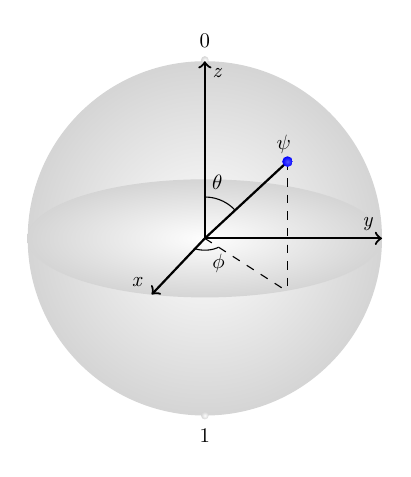
\begin{tikzpicture}[scale=0.75, transform shape]

\draw[dashed] (3,3) -- (3,0);

\shade[inner color={rgb:black,1;white,200} ,outer color={rgb:black,1;white,5}  ] (3,3) circle (3cm);
\shade[inner color={rgb:black,1;white,200} ,outer color={rgb:black,1;white,5}  ]  (3,3) ellipse (3cm and 1cm);

\shade[inner color={rgb:black,1;white,200} ,outer color={rgb:black,1;white,5}  ]  (3,6.02) circle (0.065cm);

\draw (3,6.1) node[anchor=south] {\textit{$ \ket{0}$}} ;
\draw (3,-0.1) node[anchor=north] {\textit{$ \ket{1}$}} ;

\draw[thick,->] (3,3) -- (3,6)  node[anchor=north west] {\textit{z}} ;
\draw[thick,->] (3,3) -- (6,3) node[anchor= south east] {\textit{y}} ;
\draw[thick,->] (3,3) -- (2.1,2.05) node[anchor= south east] {\textit{x}} ;

\draw[thick] (3,3) -- (4.4,4.3)  node[anchor= south] {\textit{$ \ket{\psi}$ } } ;

\draw [domain=43.8:90] plot ({3 + 0.7*cos(\x)}, {3 + 0.7*sin(\x)}) node[anchor= south west]  {\textit{$\theta$}};
\draw [domain=240:312] plot ({3 + 0.35*cos(\x)}, {3 + 0.2*sin(\x)}) node[anchor= north]  {\textit{$\phi$}};
 
\draw[dashed] (4.4,4.3) -- (4.4,2.1) ;
\draw[dashed] (4.4,4.3) -- (4.4,2.1) ;
\draw[dashed] (3,3) -- (4.4,2.1) ;

\shade[inner color={rgb:blue,2;white,1} ,outer color={rgb:blue,3}  ] (4.4,4.3) circle (0.09cm);

\shade[inner color={rgb:black,1;white,200} ,outer color={rgb:black,1;white,5}  ]   (3,0) circle (0.065cm);

\end{tikzpicture}
\captionof{figure}{Bloch sphere representation of a qubit. It is a unitary sphere, where the numbers $\theta$ and $\phi$ identify a point. The $\hat{z}$ unit vector represents the $\ket{0}$ state and $-\hat{z}$ the $\ket{1}$ state.}
\label{BlochSphere}
\end{center}
%%%%%%%%%%%%%%%%%%%

\subsection{Many qubit systems representation} 

Let us consider now a system of  \textit{n} distinguishable qubits. This system lives in a Hilbert space given by the tensor product of the Hilbert spaces of the single qubits $\mathcal{H}_i$:
\begin{equation}
\mathcal{H}= \mathcal{H}_1 \otimes \mathcal{H}_2 \otimes \dots \otimes \mathcal{H}_n
\label{3_2_firstchapter}
\end{equation}

\noindent Computational basis states of such a system are built by tensor products of each qubit basis vectors, namely $\{ \ket{j}_i \} _{i=1,\dots,n}$. A generic state $\ket{\psi} \in \mathcal{H}$ can be written as (\ref{3_3_firstchapter}).

\begin{equation}
\ket{\psi}= \sum_{\vec{j}} c_{\vec{j}} \ket{j}_1 \ket{j}_2 \dots \ket{j}_n \qquad \text{with} \quad  \sum_{\vec{j}} |c_{\vec{j}}|^2 = 1
\label{3_3_firstchapter}
\end{equation}

\noindent Therefore, a generic basis state of a many qubit system takes the form $\ket{x_1  x_2  \dots x_n}$ where $x_i \in \{0,1\}$. For $n$ qubits, the Hilbert space has dimensions $d=2^n$. 
Let's consider an example of a two qubits system: a computational basis is thus in $\{\ket{00},\ket{01},\ket{10},\ket{11}\}$, where the states are represented by the vectors in \ref{4_firstchapter}.

\begin{equation}
\ket{00} = \begin{pmatrix} 1 \\ 0 \\ 0 \\ 0 \end{pmatrix} \hspace{1cm} \ket{01} = \begin{pmatrix} 0 \\ 1 \\ 0 \\ 0  \end{pmatrix} \hspace{1cm} \ket{10} = \begin{pmatrix} 0 \\ 0 \\ 1 \\ 0  \end{pmatrix} \hspace{1cm} \ket{11} = \begin{pmatrix} 0 \\ 0 \\ 0 \\ 1  \end{pmatrix}.
\label{4_firstchapter}
\end{equation}
 
\noindent A generic state $\ket{\psi}$ of this system is given by a superposition of these four states:

\begin{equation}
 \ket{\psi}= \alpha_{00} \ket{00} +  \alpha_{01} \ket{01} +  \alpha_{10} \ket{10} +  \alpha_{11} \ket{11} \qquad \text{with} \quad  \sum_{x \in \{0,1\}^2} \abs{\alpha_x}^2 =1 
\label{5_firstchapter}
 \end{equation}

\noindent where the label $x$ encodes the basis vector for the two qubits.


\subsection{Measurements}  

In quantum mechanics, an observable $\hat{A}$ it is represented by an Hermitian operator and its average value for a generic state $\ket{\psi}$ is obtained by $\langle \hat{A} \rangle_\psi= \frac{\bra{\psi}\hat{A}\ket{\psi} }{\norm{\psi}^2}$. In practice, the value of
expectation is achieved by repeating the measurement process several times over copies of the same initial state. 
The process of measurement consists on an interaction with an external physical system which plays the role of the measurement apparatus and the observable in this case is $\hat{\sigma_z}$, whose eigenstate are $\ket{0}$ and $\ket{1}$.
 Supposing a generic state of a single qubit $\ket{\psi}=\alpha \ket{0} + \beta \ket{1}$ with $\alpha,\beta \in \mathbb{C}$, a projective measurement will make the system collapses in the states $\ket{0}$ or $\ket{1}$ with probability $|\alpha|^2$ or $|\beta|^2$, respectively. The measurement either takes the value 0 if the qubit is measured in the state $\ket{0}$, and value 1 if the qubit is measured in the state $\ket{1}$. So, it is important to keep in mind that measurement is an irreversible operation, destroying quantum information and converting it into classical information. 

A projective measurement is denoted in a quantum circuit using a 'meter' symbol, shown in Figure \ref{MeterSymbol}. This symbol will be clearer in the next sections.

\begin{center}
\[ \Qcircuit @C=1em @R=1.2em @!R {
& \qw & \meter& \qw & \qw 
} \]
 \captionof{figure}{Meter symbol in a quantum circuit.}
\label{MeterSymbol}
\end{center}


\section{Density matrix}  %S%%%%%%%%%%%%%%%%%%%%%%%%%%%%%%%%%%%%%%%%%%%%%%%%%%%%%%%%%%%%%%%%%%%%

In this section, we introduce an alternative formulation for describing quantum states: the \textit{density matrix} representation. Firstly, we focus on single-qubit isolated system, whose state is completely known. 
The states relative to isolated systems are said to be \textit{pure}; their density matrix carries all the information about the state. If the system interacts with an external environment, the state of the system is not pure anymore and it is said to be \textit{mixed}. We characterize the density matrix for a mixed state, then we focus on density matrix definition and properties; we define the \textit{reduced density matrix}, an indispensable tool in the analysis of composite quantum systems. Then we introduce the notion of \textit{entanglement}. Finally, we define the evolution of quantum states. 


\subsection{From pure states to mixed states}
A generic state $\ket{\psi}$ of a single qubit can be described in the density matrix representation:

\begin{equation}
\rho(\theta,\phi)= \ket{\psi}\bra{\psi}= 
\begin{pmatrix}
\cos^2{\frac{\theta}{2}}  &  \cos{\frac{\theta}{2}}\sin{\frac{\theta}{2}}e^{-i\phi} \vspace{0.1cm} \\ 
\cos{\frac{\theta}{2}}\sin{\frac{\theta}{2}}e^{-i\phi}   & \sin^2{\frac{\theta}{2}} 
\end{pmatrix} .
\label{7_firstchapter}
\end{equation}

\noindent This state is completely characterized, so it is called \textit{pure}. In this case, this alternative formulation is mathematically equivalent to the state vector approach used before.

It is possible to rewrite this matrix in the basis formed by identity matrix and the Pauli matrices  using the spherical coordinates\footnote{ The spherical coordinates are: $\{x=\sin \theta \cos \phi, y=\sin \theta \sin \phi, z= \cos \theta\}$}:

\begin{equation}
\rho = \frac{1}{2}
\begin{pmatrix}
1+z &  x-iy \\ 
x+iy  & 1-z
\end{pmatrix} = \frac{1}{2} (\mathbb{1} + x \hat{\sigma_x} + y \hat{\sigma_y} + z \hat{\sigma_z} )
\label{7_2_firstchapter}
\end{equation}

\noindent Now, let us suppose that a system initially in a pure state interacts with an external environment, where the environment is meant to be something outside the system\footnote{We will do a deeper analysis of system-environment interaction in the section \ref{QuantumChannels}, where we define the quantum channels.}. After the interaction, part of the information relative to the state is lost; we can only infer the probabilities relative to some measurements. The new state is said to be \textit{mixed}.

\subsection{Density matrix formalism and properties}
Mixed states are described by the density matrix formalism. Consider a quantum system among a number of states $\ket{\psi_i}$, with respective probabilities $p_i$. The \textit{density matrix} of the system is defined by the equation:

\begin{equation}
 \rho = \sum_i p_i \ket{\psi_i}\bra{\psi_i} 
 \label{8_firstchapter}
 \end{equation}
 
\noindent
The properties of the density matrix $\rho$ are:

\begin{enumerate}

\item $\rho$ is a hermitian operator. In matrix elements representation it means $\rho_{ij}=\rho_{ji}^*$.
\item $\tr \rho = 1$.
\item $\rho$ is a positive operator, i.e. $\forall  \ket{\psi}$ is $\bra{\psi} \rho \ket{\psi} \geq 0 $.

\end{enumerate}

\noindent If it exists $\ket{\psi}$ such that it is possible to write $\rho= \ket{\psi}\bra{\psi}$, a quantum system is in a \textit{pure state}, otherwise $\rho$ describes a \textit{mixed state}; it is said to be a mixture of the different pure states in the ensamble for $\rho$. 
Another way for distinguishing between the two types of states is analyzing the $\tr (\rho^2)$ \footnote{The trace operation is defined as $\tr (B) = \sum_{j=1}^{\text{dim}\, \mathcal{H}} \bra{\chi_j}B \ket{\chi_j}$, where $\{ \ket{\chi_k} \}_{k=1,\dots,\text{dim}\, \mathcal{H}}$ is an ortonormal basis of the Hilbert space.} , also called \textit{purity} of the state. If $\tr (\rho^2) = 1$ the system is in a \textit{pure state}, if $\tr (\rho^2) < 1$ it is in a \textit{mixed state}.

Consider a single qubit system, an arbitrary density matrix for a mixed state may be written in the Bloch sphere representation \cite{Nielsen} as:

 \begin{equation}
\rho = \frac{ \mathbb{1} + \vec{r} \cdot \vec{\sigma} }{2}
\label{8_2_firstchapter}
\end{equation}


\noindent where $\vec{r}$ is a real three-dimensional vector such that $\norm{ \vec{r} } \leq 1$, called the \textit{Bloch vector} for the state $\rho$. The state $\rho$ is \textit{pure} if and only if $\norm{ \vec{r} } =1$. Therefore, the possible density matrices for a single qubit system, that are generic vectors on the Bloch sphere, correspond to pure states ($\norm{ \vec{r} } =1$), while the vectors inside the sphere correspond to mixed states.

Consider the matrix $\rho$, the diagonal terms are called \textit{terms of population}, while the terms outside the diagonal are the \textit{terms of coherence}. The last one describes correlations between the single states.




\subsection{Reduced density matrix}

Let us consider two physical systems $A$ and $B$, whose state is described by the density matrix $\rho^{AB}$. Let us suppose the reduced density matrix for system $A$ is defined by:

\begin{equation}
\rho^A = \underset{B}\tr  (\rho^{AB})
 \label{11_firstchapter}
\end{equation}

\noindent where $\underset{B}\tr$ is called \textit{partial trace} over the system $B$.

If $\{ \ket{a_k} \}_{i=1,\dots,m}$ and $\{ \ket{b_l} \}_{j=1,\dots,p}$ are orthonormal bases for the systems $A$ and $B$  respectively, the \textit{partial trace} of $A$ over the system $B$ is obtained by summing only over the basis vector of $B$, namely:

\begin{equation}
(\rho^A)_{ij} = ( \underset{B}\tr \rho^{AB} )_{ij} = \sum_l^{p} \bra{b_l} \rho^{AB} \ket{b_l} = \sum_l^{p} \rho_{i b_l}^{j b_l} \ket{i} \bra{j}
 \label{12_firstchapter}
\end{equation}

\noindent The reduced density matrix operation do not preserve the \textit{purity} of the state. It means that if $\rho^{AB}$ represents a pure state, then $\rho^A$ or $\rho^B$ could be mixed.




\subsection{Entanglement} 
\label{Concurrence_theory}
The entanglement is a genuine quantum phenomenon that entails an intrinsic correlation between the constituents of a quantum system.
This concept could be understood considering as example a 'quantum book' \cite{PreskillNote},  a book whose pages are not to be read individually, because the information in that quantum book is not imprinted on the individual pages; it is encoded almost entirely in how the pages are correlated with one another . 

An entangled state of a quantum system is characterized by the fact that its state cannot be factorized as a tensor product of states of its local constituents. An entangled state can be written as:

\begin{equation}
(\rho^{AB}) = \sum_i p_i (\rho_i^A \otimes \rho_i^B).
 \label{13_firstchapter}
\end{equation}

\noindent
Now, let's consider few examples:

\begin{itemize}
\item  for a two-qubit system a type of entangled states are the \textit{Bell states}, represented as
\begin{equation}
\ket{\phi^+} = \frac{ \ket{00}+\ket{11} }{\sqrt{2}} \qquad \ket{\phi^-} = \frac{ \ket{00}-\ket{11} }{\sqrt{2}} \qquad \ket{\psi^+} = \frac{ \ket{01}+\ket{10} }{\sqrt{2}} \qquad \ket{\psi^-} = \frac{ \ket{01}-\ket{10} }{\sqrt{2}}
 \label{14_firstchapter}
\end{equation}

\item for a system of $N > 2$ qubits, an important entangled state is the Greenberger–Horne–Zeilinger state (\textit{GHZ state}), that has the form
\begin{equation}
\ket{\text{GHZ}}= \frac{\, \, \ket{0}^{\otimes N} + \ket{1}^{\otimes N} }{\sqrt{2} }.
 \label{15_firstchapter}
\end{equation}
\noindent The importance of these states is that the GHZ states are maximally entangled quantum states. They can be used for estimating the fidelity of the gate operations as we will see in Chapter \ref{chapter3}.
\end{itemize}




\subsubsection{How to quantify entanglement}

In order to quantify the entanglement, we introduce the Von Neumann \textit{entropy} associated to a density matrix $\rho$:

\begin{equation}
S(\rho) \equiv - \tr(\rho \log_2 \rho)
 \label{16_firstchapter}
\end{equation}

\noindent If $\rho_{AB}$ is a pure state which describes the state of the systems A and B, a good measurement of entanglement is the entropy of Von Neumann of the reduced density matrix of one of the two subsystems, for instance: 
\begin{equation}
E(\rho)= S(\rho_A) .
 \label{17_firstchapter}
\end{equation}

\noindent If instead the state $\rho$ is mixed we have to modify the previous definition: let us consider the mixed state $\rho_{AB} = \sum_{j=1}^k p_j \ket{\psi_j}\bra{\psi_j}$ where $ \{\ket{\psi_j}\}$ are basis of $\mathcal{H_{\text{AB}}}$. 
 A measurement of entanglement is
 
 \begin{equation}
E(\rho) \equiv \min_{ \ket{\psi_j}\bra{\psi_j} }\, \sum_{i=1}^k p_i S(\rho_A^i)  
\label{18_firstchapter}
\end{equation}

\noindent where the count is done for all families $\{ \ket{\psi_j}\bra{\psi_j} \}$ of states of $\rho_{AB}$.

If we consider a two-qubit system, an entanglement measurement can by done using the \textit{concurrence} method \cite{Concurrence}. The \textbf{concurrence} is defined for a state $\rho$ of two qubits as:
 \begin{equation}
 {\mathcal  {C}}(\rho )\equiv \max(0,\lambda _{1}-\lambda _{2}-\lambda _{3}-\lambda _{4})
\label{18_2_firstchapter}
\end{equation}

\noindent in which $\lambda _{1},...,\lambda _{4}$ are the eigenvalues, in decreasing order, of the Hermitian matrix

\begin{equation}
%R={\sqrt  {{\sqrt  {\rho }}{\tilde  {\rho }}{\sqrt  {\rho }}}}
R=  \rho \tilde  {\rho }
\label{18_3_firstchapter}
\end{equation}

\noindent with

\begin{equation}
{\tilde  {\rho }}=(\sigma _{{y}}\otimes \sigma _{{y}})\rho (\sigma _{{y}}\otimes \sigma _{{y}}).
\label{18_4_firstchapter}
\end{equation}


\subsection{Density matrix evolution}
The evolution of the density matrix $\rho$ is described by the \textit{Liouville-von Neumann} equation:

\begin{equation}
i \hbar \dev{\rho(t)}{t} = [H,\rho(t)].
\label{9_firstchapter}
\end{equation}

\noindent The evolution of a quantum system, that can be either closed or open, can be described also by the quantum operation formalism. Suppose that the system is in the state $\rho$, the quantum state transforms as 
\begin{equation}
\rho'= \mathcal{E}(\rho)
 \label{10_2_firstchapter}
 \end{equation}
 
\noindent where the map $\mathcal{E}$ is known as \textit{quantum operation} \cite{Nielsen}.

 
 \subsubsection{Closed quantum systems}
 
Suppose we have a closed quantum system whose evolution is described by the unitary operator $\hat{U}$. The evolution of the density operator is described by the equation:
\begin{equation}
 \rho(t)= \mathcal{E}(\rho) \equiv \hat{U} \rho \hat{U}^\dagger 
 \label{10_firstchapter}
 \end{equation}
 
 \noindent
The unitary evolution preserves the \textit{purity} of the state. It means that a pure state can unitary evolve only to pure states and at the same way a mixed state evolves only to mixed states (only if the system remains closed). The unitary evolution can be represented as a circuit model, as shown in Figure \ref{closed_system}.

\begin{center}
\[ \Qcircuit @C=1em @R=1.2em @!R {
\lstick{\rho} & \qw & \gate{\hat{U}} & \qw & \qw & \rstick{\hspace{-0.5cm} \hat{U} \rho \hat{U}^\dagger  } 
} \]
\captionof{figure}{\label{closed_system} Circuit model of closed quantum system.}
\end{center}

 \subsubsection{Open quantum systems}
 
 Consider a system, called the \textit{principal system}, interacting with an \textit{environment}. The system is said to be open due to its interaction with the environment. The dynamics of such a quantum system   $\rho(t=0) = \rho_S \otimes \rho_E $  can be described as:
 
  \begin{equation}
  \rho(t) = \mathcal{E}(\rho_S) \equiv \underset{E}\tr [ \hat{U} ( \rho_S \otimes \rho_E) \hat{U}^\dagger ] 
  \label{10_3_firstchapter}
 \end{equation}
 

 
Now, we describe the evolution of an open system. Consider a system defined by the state $\rho= \rho_S \otimes \rho_E$, that is the tensor product of the \textit{principal system} state and the \textit{environment} state. The dynamics of such a quantum system could be described as arising from an interaction between these two systems, which together form the closed quantum system $\rho$. In other words,  suppose to have a system $\rho_S$, which is sent into a box which is coupled to the environment $\rho_E$. This coupling is described by the action of the $\hat{U}$ operation. After the gate application, the system no longer interacts with the environment and we can perform the partial trace over the environment to obtain the reduced state of $\rho_S$, namely:


 \noindent
 The dynamics of the open quantum system is modeled in Figure \ref{open_system}.
 
 \begin{center}
\[ \Qcircuit @C=1em @R=1.2em @!R {
\lstick{\rho_S} & \qw & \multigate{1}{\hat{U}} & \qw & \qw & \rstick{\hspace{-0.5cm}  \mathcal{E}(\rho_S)  }  \\
\lstick{\rho_E} & \qw & \ghost{\hat{U}} & \qw & \qw & 
} \]
\captionof{figure}{\label{open_system} Circuit model of open quantum systems. An open quantum system consists of two parts: $\rho_S$, the principal system, and $\rho_E$ the environment system.}
\end{center}

 
Moreover, we can analyze the open quantum systems evolution representing quantum operations in the \textit{Kraus representation} \cite{Benenti}. Let $\{\ket{e_k}\}$ be an orthonormal basis for the state space of the environment and $\ket{e_0}$ its initial state; it is possible to write: 
\begin{equation}
 \mathcal{E}(\rho_S) = 
  \sum_k E_k \rho_S E_k^\dagger  \quad \text{with} \quad \sum_k E_k^\dagger E_k = 1 
  \label{10_3_firstchapter}
 \end{equation}

\noindent where $E_k \equiv \bra{e_k}U\ket{e_0}$ is an operator on the state space of the principal system. The operators $\{ E_k \}$ are known as \textit{Kraus operators} and they are not unique. 







\section{Quantum computation}  

The information carried by quantum states can be manipulated by using quantum gates. 
They are the building blocks of quantum circuits, as well as classical logic gates for conventional digital circuits. 
A quantum circuit is constituted by a discrete sets of components which describe a computational procedure. We suppose to consider a system of $n$ qubits, let's describe the main steps to realize a quantum circuit:

\begin{enumerate}

\item First, each qubit is initialized in a quantum state. Generally, the initial state of a qubit is chosen as $\ket{0}$, the ground state.

\item Lines are drawn in the circuit to represent \textit{wires} in the quantum circuit and they represent also the flux of time from left to right.

\item Quantum gates $\hat{U}$ can be applied to one or more qubits. 

\item Finally, the quantum states could be measured by measurement operation.

\end{enumerate}

A general example of a $n$ qubits system is shown in Figure \ref{ExampleCircuit}; it is important to underline that a circuit has to be read from left-to-right.

\begin{center}

\[ 
\Qcircuit @C=1.6em @R=1.2em {
& & &\lstick{\ket{0}} & \qw & \multigate{3}{\hat{U_1}} & \qw & \gate{\hat{U_2}}  & \qw & \meter \\
n & & & \lstick{\ket{0}} & \qw & \ghost{\hat{U_1}} & \qw & \qw & \qw & \meter \\
qubits & & & \lstick{ \vdots \ }& \cdots & \nghost{\hat{U_1}} & \cdots & \cdots  & \cdots & \vdots \\
& & & \lstick{\ket{0}}& \qw &  \ghost{U_1} & \gate{\hat{U_3}} & \qw & \qw & \meter
%\inputgroupv{1}{4}{2.8em}{2.8em}{ }
\gategroup{1}{3}{4}{3}{2.3em}{\{}
}
 \]
 
 \captionof{figure}{An example of a generic quantum circuit of $n$ qubits. The qubits are initialized in the state $\ket{0}$. A $n$ qubits gate is applied on all qubits and other gates are applied randomly. Finally all the qubits are measured.}
\label{ExampleCircuit}

\end{center}


Quantum gates are represented by unitary matrices generically indicated by $\hat{U}$. 
As we will see later, this assumption is valid when the system is isolated.
Let us stress that unitarity property makes a quantum gate reversible: input and output for a given number of qubits gate must be equal; a gate which acts on $n$ qubits is represented by a $2^{n}\times 2^{n}$ unitary matrix, namely the dimension of the Hilbert space.

The action of the quantum gate is given by the product of the matrix representing the gate with the vector which represents the quantum state:
 
 \begin{equation}
  \ket{\psi '}= \hat{U} \ket{\psi}.
  \label{6_firstchapter}
  \end{equation}
 
 \noindent We illustrate now some quantum gates: single and two-qubits gates. Gates involving more qubits can be decomposed in terms of these ones.
We show in particular the gates $u_1, u_2, u_3$, which are the native gates implemented on the IBM devices, as we will discuss later in Chapter \ref{chapter2}.
For each gate we show the symbol used for representing it in the circuits.

 
\subsection{Single qubit gates}  %SUB%%%%%%%%%%%%%%%%%%%%%%%%%%%%%%%%%%%%%%%%%%%%%%%%%%%%%%%%%%%%%%%%%%%%
A gate which acts on a single qubit is represented by a $2\times 2$ unitary matrix $\hat{U}$. The most general form of a single qubit unitary matrix \cite{TutorialQiskit}  is:

\begin{equation}
 \hat{U}(\theta,\phi,\lambda) = \begin{pmatrix}
\cos(\theta/2) & -e^{i\lambda}\sin(\theta/2) \\
e^{i\phi}\sin(\theta/2) & e^{i\lambda+i\phi}\cos(\theta/2) 
\end{pmatrix}.
\label{U_general_gate}
\end{equation}

\noindent where $0\leq \theta \leq \pi$, $0\leq \phi < 2\pi$ and  $0\leq \lambda < 2 \pi$.

\noindent Now, let's illustrate the most common gates.

\subsubsection{Identity gate} %%%%%%%%%%%%%%%
The Identity gate is a single qubit operation that leaves a generic state $\ket{\psi}$ unchanged:

\begin{equation}
 \mathbb{I}=\hat{U}(0,0,0) = \begin{pmatrix}
1 & 0 \\
0 & 1
\end{pmatrix} \hspace{1cm}
\Qcircuit @C=1em @R=.7em {
&\qw & \gate{\mathbb{I}} & \qw & \qw
}  
\label{IdentityGate}
\end{equation}
 %\captionof{figure}{Identity gate.}

\subsubsection{Pauli gates}  %%%%%%%%%%%%%%%

\begin{itemize}
\item \textcolor{blue}{\textbf{X: Bit-flip gate}} \\ %%%%%%%%%%%%%%%%%
The Pauli-X gate is a single-qubit $\pi$ rotation around the x-axis:

\begin{equation}
 X=\hat{U}(\pi,0,\pi) = 
\begin{pmatrix}
0 & 1 \\
1 & 0
\end{pmatrix} \hspace{1cm}
\Qcircuit @C=1em @R=.7em {
&\qw & \gate{X} & \qw & \qw
}  
\label{XGate}
\end{equation}

\noindent It maps $\ket{0}$ to $\ket{1}$ and $\ket{1}$ to $\ket{0}$.
It is possible to visualize how the X-gate acts on an input state $\ket{\psi}=\ket{0}$, in the Bloch sphere representation in Figure \ref{XBlochSphere}. 
%%%FIGURA SFERA DI BLOCH PER X %%%
\begin{center}

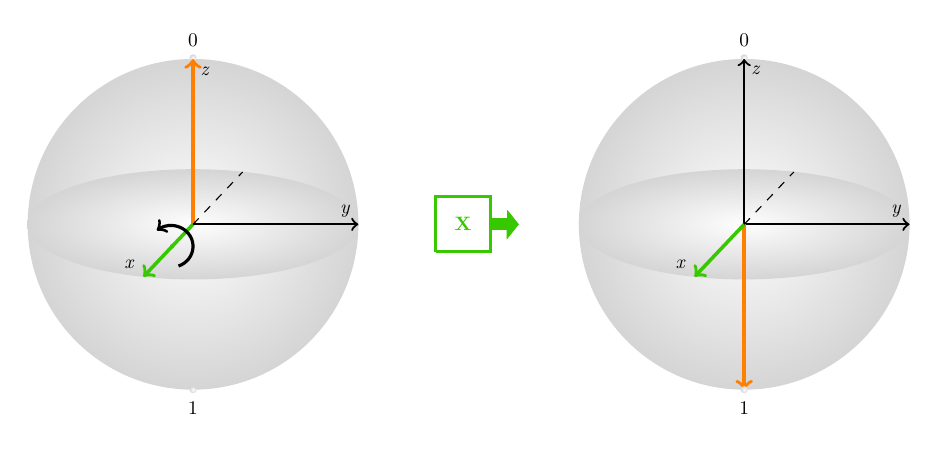
\begin{tikzpicture} [scale=0.7, transform shape]

\draw[dashed] (3,3) -- (3,0);

\shade[inner color={rgb:black,1;white,200} ,outer color={rgb:black,1;white,5}  ] (3,3) circle (3cm);
\shade[inner color={rgb:black,1;white,200} ,outer color={rgb:black,1;white,5}  ]  (3,3) ellipse (3cm and 1cm);
%\draw (3,3) circle (3cm);
%\draw[dashed, color={rgb:black,1;white,2}] (3,3) ellipse (3cm and 1cm);

\shade[inner color={rgb:black,1;white,200} ,outer color={rgb:black,1;white,5}  ] (3,6.02) circle (0.065cm);

\draw (3,6.1) node[anchor=south] {\textit{$ \ket{0}$}} ;
\draw (3,-0.1) node[anchor=north] {\textit{$ \ket{1}$}} ;

\draw[color=orange,line width=0.45mm,->] (3,3) -- (3,6)  node[text=black,anchor=north west] {\textit{z}} ;
\draw[thick,->] (3,3) -- (6,3) node[anchor= south east] {\textit{y}} ;
\draw[color={rgb:red,60;green,216},line width=0.45mm,->] (3,3) -- (2.1,2.05) node[text=black,anchor= south east] {\textit{x}} ; %%green

\draw[dashed] (3,3) -- (3.9,3.95)  ;

\shade[inner color={rgb:black,1;white,200} ,outer color={rgb:black,1;white,5}  ] (3,0) circle (0.065cm);

%%%%

\coordinate (birds) at (8-0.1,3);
\node[text={rgb:red,60;green,216}] at (birds) {\textbf{X}};

\draw[line width=0.40mm, color={rgb:red,60;green,216}] (7.5-0.1,2.5) -- (8.5-0.1,2.5) -- (8.5-0.1,3.5) -- (7.5-0.1,3.5) -- (7.5-0.1,2.5) ;

%freccia
\filldraw[ color={rgb:red,60;green,216}] (8.5-0.1,2.9) -- (8.8-0.1,2.9) -- (8.8-0.1,3.1) -- (8.5-0.1,3.1) -- (8.5-0.1,2.9) ;

\filldraw[ color={rgb:red,60;green,216}] (8.8-0.1,2.9) -- (8.8-0.1,2.75) --  (9-0.1,3) -- (8.8-0.1,3.25);

%%%SFERA TRASLATA%%
\draw[dashed] (3+10,3) -- (3+10,0);

\shade[inner color={rgb:black,1;white,200} ,outer color={rgb:black,1;white,5}  ] (3+10,3) circle (3cm);
\shade[inner color={rgb:black,1;white,200} ,outer color={rgb:black,1;white,5}  ]  (3+10,3) ellipse (3cm and 1cm);
%\draw (3,3) circle (3cm);
%\draw[dashed, color={rgb:black,1;white,2}] (3,3) ellipse (3cm and 1cm);

\shade[inner color={rgb:black,1;white,200} ,outer color={rgb:black,1;white,5}  ] (3+10,6.02) circle (0.065cm);

\draw (3+10,6.1) node[anchor=south] {\textit{$ \ket{0}$}} ;
\draw (3+10,-0.1) node[anchor=north] {\textit{$ \ket{1}$}} ;

\draw[color=black,thick,->] (3+10,3) -- (3+10,6)  node[text=black,anchor=north west] {\textit{z}} ;

\draw[thick,->] (3+10,3) -- (6+10,3) node[anchor= south east] {\textit{y}} ;

\draw[line width=0.45mm,color=orange,->] (3+10,3) -- (3+10,0) ; %%orange
\draw[color={rgb:red,60;green,216},line width=0.45mm,->] (3+10,3) -- (2.1+10,2.05) node[text=black,anchor= south east] {\textit{x}} ; %%green

\draw[dashed] (3+10,3) -- (3.9+10,3.95)  ;

\shade[inner color={rgb:black,1;white,200} ,outer color={rgb:black,1;white,5}  ] (3+10,0) circle (0.065cm);




%%rotazione
\draw [line width=0.40mm,domain=-70:130,->] plot ({2.6 + 0.4*cos(\x)}, {2.6 + 0.38*sin(\x)});
\shade[inner color={rgb:red,60;green,216} ,outer color={rgb:red,60;green,216}  ] (2.62,2.6) circle (0.04cm);


\end{tikzpicture}

\captionof{figure}{Visualization of the bit-flip gate on the Bloch sphere, acting on the input state $\ket{0}$. The gate maps the input state $\ket{0}$ to the $\ket{1}$ state and viceversa.}
\label{XBlochSphere}
\end{center}
%%%%%%%%%%%%%%%%%%%



\item \textcolor{blue}{\textbf{Y: Bit-and phase-flip gate}} \\ %%%%%%%%%%%%%%%%%
The Pauli-Y gate is a single-qubit  $\pi$ rotation around the y-axis:

\begin{equation}
 Y=\hat{U}(\pi,\pi/2,\pi/2) = 
\begin{pmatrix}
0 & -i \\
i & 0
\end{pmatrix} \hspace{1cm}
\Qcircuit @C=1em @R=.7em {
&\qw & \gate{Y} & \qw & \qw
}  
\label{YGate}
\end{equation}

\noindent It maps $\ket{0}$ to $i\ket{1}$ and $\ket{1}$ to $-i\ket{0}$.

\item \textcolor{blue}{\textbf{Z: Phase-flip gate}} \\ %%%%%%%%%%%%%%%%%
The Pauli-Z gate is a single-qubit $\pi$ rotation around the z-axis:

\begin{equation}
 Z =\hat{U}(0, 0,\pi) = 
\begin{pmatrix}
1 & 0 \\
0 & -1
\end{pmatrix} \hspace{1cm}
\Qcircuit @C=1em @R=.7em {
&\qw & \gate{Z} & \qw & \qw
}  
\label{ZGate}
\end{equation}

\noindent It leaves the basis state $\ket{0}$ unchanged and maps $\ket{1}$ to $-\ket{1}$.
 
\end{itemize}


\subsubsection{Hadamard gate}  %%%%%%%%%%%%%%%
The Hadamard gate is a single-qubit operation that maps the basis state $\ket{0}$ to $\frac{(\ket{0}+\ket{1})}{\sqrt{2}}$ and $\ket{1}$ to $\frac{(\ket{0}-\ket{1})}{\sqrt{2}}$, thus creating an equal superposition of the two:

\begin{equation}
H=\hat{U}(\pi/2,0,\pi) = \frac{1}{\sqrt{2}}
\begin{pmatrix}
1 & 1 \\
1 & -1
\end{pmatrix} \hspace{1cm}
\Qcircuit @C=1em @R=.7em {
&\qw & \gate{H} & \qw & \qw
}  
\label{HGate}
\end{equation}

\noindent As the gates X,Y,Z, also the Hadamard one implements a rotation on the Bloch sphere. The difference is that it rotates around an axis located halfway between x and z in the plane $\bot$ to y, as we show in Figure \ref{HBlochSphere}. Here, the input state $\ket{0}$ is rotated by $\pi$ angle around the $\frac{\hat{x}+\hat{z}}{2}$ axis into the $\frac{(\ket{0}+\ket{1})}{\sqrt{2}}$ state.



%%%FIGURA SFERA DI BLOCH PER H %%%
\begin{center}
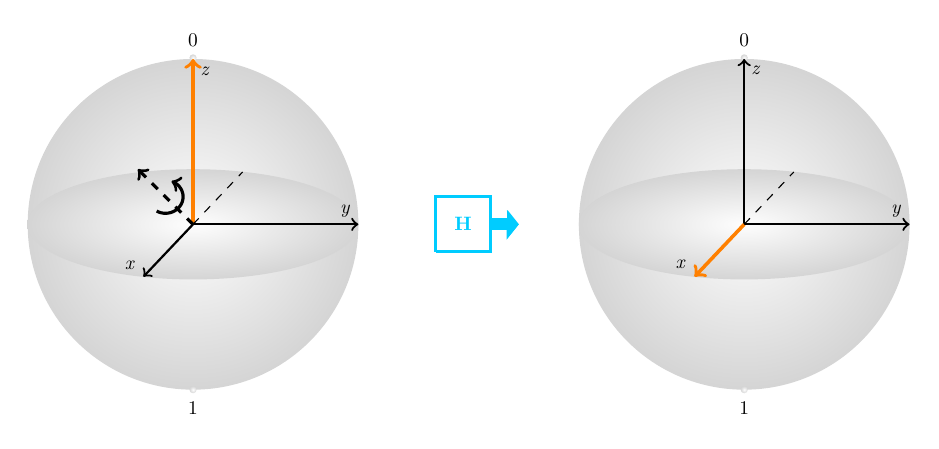
\begin{tikzpicture}[scale=0.7, transform shape]

\draw[dashed] (3,3) -- (3,0);

\shade[inner color={rgb:black,1;white,200} ,outer color={rgb:black,1;white,5}  ] (3,3) circle (3cm);
\shade[inner color={rgb:black,1;white,200} ,outer color={rgb:black,1;white,5}  ]  (3,3) ellipse (3cm and 1cm);
%\draw (3,3) circle (3cm);
%\draw[dashed, color={rgb:black,1;white,2}] (3,3) ellipse (3cm and 1cm);

\shade[inner color={rgb:black,1;white,200} ,outer color={rgb:black,1;white,5}  ] (3,6.02) circle (0.065cm);

\draw (3,6.1) node[anchor=south] {\textit{$ \ket{0}$}} ;
\draw (3,-0.1) node[anchor=north] {\textit{$ \ket{1}$}} ;

\draw[color=orange,line width=0.45mm,->] (3,3) -- (3,6)  node[text=black,anchor=north west] {\textit{z}} ;
\draw[thick,->] (3,3) -- (6,3) node[anchor= south east] {\textit{y}} ;
\draw[color=black,thick,->] (3,3) -- (2.1,2.05) node[text=black,anchor= south east] {\textit{x}} ;

\draw[dashed] (3,3) -- (3.9,3.95)  ;

\shade[inner color={rgb:black,1;white,200} ,outer color={rgb:black,1;white,5}  ] (3,0) circle (0.065cm);

%%%%

\definecolor{yucky}{HTML}{00CCFF}

\coordinate (birds) at (8-0.1,3);
\node[text=yucky] at (birds) {\textbf{H}};

\draw[line width=0.40mm, color=yucky] (7.5-0.1,2.5) -- (8.5-0.1,2.5) -- (8.5-0.1,3.5) -- (7.5-0.1,3.5) -- (7.5-0.1,2.5) ;

%freccia
\filldraw[ color=yucky] (8.5-0.1,2.9) -- (8.8-0.1,2.9) -- (8.8-0.1,3.1) -- (8.5-0.1,3.1) -- (8.5-0.1,2.9) ;

\filldraw[ color=yucky] (8.8-0.1,2.9) -- (8.8-0.1,2.75) --  (9-0.1,3) -- (8.8-0.1,3.25);

%%%SFERA TRASLATA%%
\draw[dashed] (3+10,3) -- (3+10,0);

\shade[inner color={rgb:black,1;white,200} ,outer color={rgb:black,1;white,5}  ] (3+10,3) circle (3cm);
\shade[inner color={rgb:black,1;white,200} ,outer color={rgb:black,1;white,5}  ]  (3+10,3) ellipse (3cm and 1cm);
%\draw (3,3) circle (3cm);
%\draw[dashed, color={rgb:black,1;white,2}] (3,3) ellipse (3cm and 1cm);

\shade[inner color={rgb:black,1;white,200} ,outer color={rgb:black,1;white,5}  ] (3+10,6.02) circle (0.065cm);

\draw (3+10,6.1) node[anchor=south] {\textit{$ \ket{0}$}} ;
\draw (3+10,-0.1) node[anchor=north] {\textit{$ \ket{1}$}} ;

\draw[color=black,thick,->] (3+10,3) -- (3+10,6)  node[text=black,anchor=north west] {\textit{z}} ;

\draw[thick,->] (3+10,3) -- (6+10,3) node[anchor= south east] {\textit{y}} ;
\draw[color=orange,line width=0.45mm,->] (3+10,3) -- (2.1+10,2.05) node[text=black,anchor= south east] {\textit{x}} ; 

\draw[dashed] (3+10,3) -- (3.9+10,3.95)  ;

\shade[inner color={rgb:black,1;white,200} ,outer color={rgb:black,1;white,5}  ] (3+10,0) circle (0.065cm);



%%rotazione
\draw [line width=0.40mm,domain=-120:70,->] plot ({2.5 + 0.32*cos(\x)}, {3.5 + 0.3*sin(\x)});
\draw [dashed,line width=0.40mm,->] (3,3) -- (2,4);

\end{tikzpicture}
\captionof{figure}{Visualization of the Hadamard gate on the Bloch sphere, starting from the input state $\ket{0}$. The state $\ket{0}$ is rotated around the $\frac{\hat{x}+\hat{z}}{2}$ axis into the $\frac{(\ket{0}+\ket{1})}{\sqrt{2}}$ state.}
\label{HBlochSphere}
\end{center}
%%%%%%%%%%%%%%%%%%%

\subsubsection{Phase-shift gate}  %%%%%%%%%%%%%%%
The Phase-shift is a single-qubit operation that leaves the basis state $\ket{0}$ unchanged and adds a relative phase on the basis state $\ket{1}$ mapping it to $e^{i\phi}\ket{1}$:

\begin{equation}
 R_z(\delta)= \hat{U}(0,0,\delta) = 
\begin{pmatrix}
1 & 0 \\
0 & e^{i \delta}
\end{pmatrix} \hspace{1cm}
\Qcircuit @C=1em @R=.7em {
&\qw & \gate{ R_z(\delta)} & \qw & \qw
} 
\label{PhaseShiftGate}
\end{equation}

\subsubsection{Native gates implemented in the IBM devices}  %%%%%%%%%%%%%%%\boldmath{$u_2$} gate
In the following chapters, we will work on the IBM quantum computers whose software implements gates in a certain form. Therefore, we illustrate the native single-qubit gates implemented in the IBM device:

\begin{equation}
u_3(\theta,\phi,\lambda) \equiv \hat{U}(\theta,\phi,\lambda) = \begin{pmatrix}
\cos(\theta/2) & -e^{i\lambda}\sin(\theta/2) \\
e^{i\phi}\sin(\theta/2) & e^{i\lambda+i\phi}\cos(\theta/2) 
\end{pmatrix}
\label{U3gate}
\end{equation}

\begin{equation}
 u2(\phi, \lambda) \equiv \hat{U}(\pi/2,\phi,\lambda) =
\frac{1}{\sqrt{2}} \begin{pmatrix}
1 & -e^{i\lambda} \\
e^{i\phi} & e^{i(\phi + \lambda)}
\end{pmatrix}
\label{U2gate}
\end{equation}

\begin{equation}
 u_1(\delta) \equiv  \hat{U}(0,0,\delta) = 
\begin{pmatrix}
1 & 0 \\
0 & e^{i \delta}
\end{pmatrix} .
\label{U1gate}
\end{equation}





\subsection{Two-qubit gates}
In this section we introduce some fundamental gates which cannot be decomposed into single-qubit gates: SWAP and controlled.

\subsubsection{SWAP gate}
The SWAP gate literally swaps the state of two qubits. 
For example, it transforms the basis vectors as 
$\left|00\right\rangle \rightarrow \left|00\right\rangle~,~\left|01\right\rangle \rightarrow \left|10\right\rangle~,~\left|10\right\rangle \rightarrow \left|01\right\rangle~,~\left|11\right\rangle \rightarrow \left|11\right\rangle$. The SWAP gate matrix representation and the relative circuit symbol are, respectively:

\begin{equation}
\mathrm{SWAP} = 
\begin{pmatrix}
1 &0 & 0 & 0\\
0 & 0 & 1 & 0\\
0 &1 & 0 & 0\\
0 & 0 & 0 & 1
\end{pmatrix} \hspace{1cm}
\Qcircuit @C=1em @R=1.2em @!R {
& \qw & \qswap & \qw & \qw\\
& \qw & \qswap  \qwx & \qw & \qw 
} 
\label{SWAPGate}
\end{equation}

\subsubsection{Controlled gates}

A common multi-qubit gate involves the application of a gate to one qubit, conditioned on the state of another qubit. 
In the controlled two-qubit gate $C_{\hat{U}}$, a unitary transformation $\hat{U}$ is applied to one of the two qubits, known as \textit{target} qubit, if the other, the \textit{control} qubit, is for example in the state $\ket{1}$. 
The most general form \cite{TutorialQiskit} is the following \footnote{We consider the basis vectors of the two-qubit system ordered as $\ket{00}$,$\ket{01}$,$\ket{10}$,$\ket{11}$.}:

\begin{equation}
C_{\hat{U}}(\theta, \phi, \lambda) \equiv 
\begin{pmatrix}
1 & 0 &0 & 0\\
0 & 1 & 0 &0\\
0 & 0 & e^{-i(\phi+\lambda)/2}\cos(\theta/2)  & -e^{-i(\phi-\lambda)/2}\sin(\theta/2)\\
0 & 0 & e^{i(\phi-\lambda)/2}\sin(\theta/2)  &e^{i(\phi+\lambda)/2}\cos(\theta/2)
\end{pmatrix}.
\label{CU_general_gate}
\end{equation}

\noindent For instance, we consider the \textbf{Controlled-X} gate that flips the target qubit when the control qubit is in the state $\left|1\right\rangle$. For example, let us suppose that the first qubit is the control one and the second is the target, therefore the CX gate maps $\ket{00}$ to $\ket{00}$ and $\ket{10}$ to $\ket{11}$. The action of the gate can be summarized as $ \ket{A,B} \rightarrow \ket{A, B \oplus A}$, where $\oplus$ is addition modulo two.
The circuit representation for the CX is the following:

\begin{equation}
 C_X = 
\begin{pmatrix}
1 & 0 & 0 & 0\\
0 & 1 &0 &0\\
0 &0 & 0 & 1\\
0 &0 &1 &0
\end{pmatrix} \hspace{1cm}
 \Qcircuit @C=1em @R=1.2em {
& \qw &\ctrl{1} & \qw & \qw \\
& \qw & \targ  & \qw & \qw
}  
\label{Controlled-NOTGate}
\end{equation}

\noindent where the fill dot represents the control qubit (upper line), while the $ \oplus$ represents the transformation applied to the target qubit (bottom line). 




%\begin{postulate} % per inserire cosa titolo tra parentesi [ titolo teorema ]
%\label{postulate3}
%Quantum measurements are described by a collection $\{ M_m \}$ of \textit{measurement operators}. These are operators acting on the state space of the system being measured. The index $m$ refers to the measurement outcomes that may occur in the experiment. If the state of the quantum system is $\ket{\psi}$ immediately before the measurements, then the probability that result $m$ occurs is given by:
%\[ p(m)=\bra{\psi}M_m^\dagger M_m \ket{\psi} \]
%and the state of the system after the measurement is
%\[ \frac{M_m \ket{\psi}}{ \sqrt{\bra{\psi}M_m^\dagger M_m \ket{\psi} } } \]
%The measurement operators satisfy the \textit{completeness equation}:
%\[ \sum_m M_m^\dagger M_m = 1 \]
%\end{postulate}
%
%An important special class of measurement is known as \textit{projective measurement}.  \\
%
%\begin{projective}
%A projective measurement is described by an \textit{observable}, $M$, a Hermitian operator on the state space of the system being observed. The observable has a spectral decomposition,
%\[ M = \sum_m m P_m \]
%where $P_m$ is the projector onto the eigenspace of $M$ with eigenvalue $m$. The possible outcomes of the measurement correspond to the eigenvalues, $m$, of the observable. Upon measuring the state $\ket{\psi}$, the probability of getting result $m$ is given by
%\[ p(m)= \bra{\psi}P_m\ket{\psi} \]
%Given that outcome $m$ occured, the state of the quantum system immediately after the measurement is 
%\[ \frac{ P_m \ket{\psi} } { \sqrt{ p(m)} } \]
%
%\end{projective}


 \subsection{Example of applications of quantum circuits}  %SUB%%%%%%%%%%%%%%%%%%%%%%%%%%%%%%%%%%%%%%%%%%%%%%%%%%%%%%


What is a quantum computer good for? Practically speaking, many interesting problems are impossible to solve on a classical computer. This is not because they are in principle insoluble, but because of the huge resources required. The spectacular promise of quantum computers is to enable new algorithms to solve problems which need resources unavailable on a classical computer. 
There are two main classes of quantum algorithms. The first class is based on the so called \textit{quantum Fourier trasnsform} \cite{Nielsen}: it includes remarkable algorithms for solving the phase estimation and factory problems, providing  a striking \textit{exponential} speedup over the best known classical algorithms. The second class of algorithms is based upon Grover's algorithm for performing \textit{quantum searching} \cite{Nielsen}. They provide a \textit{quadratic} speedup over the best possible classical algorithms. 





\section{Quantum noise: quantum channels}  %S%%%%%%%%%%%%%%%%%%%%%%%%%%%%%%%%%%%%%%%%%%%%%%%%%%%%%%%%%%%%%%%%%%%%
\label{QuantumChannels}

Quantum noise is a consequence of non-unitary effects involved in the dynamics of a system that interacts with an external environment during its dynamics. 
The \textit{Kraus representation} previously introduced must be used to model the effects of noise on quantum systems. In fact, quantum effects can be modeled by introducing a set of quantum channels that act as the evolution  $\rho \rightarrow \rho ' =  \sum_k E_k \rho E_k^\dagger$. Therefore each quantum channel is characterized by a collection of \textit{Kraus operators}.

Single qubit quantum channels can be illustrated with a geometric representation, namely an affine transformation of the coordinates of the $\rho$ state \cite{Nielsen}.
 Let us consider a mixed state $\rho$ and its representation on the Bloch sphere, an arbitrary trace-preserving quantum operation is equivalent to a map of the form:

\begin{equation}
\vec{r} \overset{\mathcal{E}} \rightarrow \vec{r'} = M \vec{r'} + \vec{c}.
\label{19_firstchapter}
\end{equation}

\noindent This affine transformation transforms the Bloch sphere in a translated ellipsoid with a minor or equal volume.
 
The related \textit{Kraus operator} has the form:

\begin{equation}
E_i = \alpha_i \mathbb{1} + \sum_{k=1}^3 a_{ik} \sigma_k
\label{20_firstchapter}
\end{equation}

\noindent where the parameters are

\begin{equation}
M_{jk}=\sum_{l=1}^3 \Bigl[ a_{lj} a_{lk}^* + a_{lj}^* a_{lk} + ( |\alpha_l |^2 - \sum_{p=1}^3 a_{lp} a_{lp}^* ) \delta_{jk} + i \sum_{p=1}^3 \epsilon_{jkp} (\alpha_l a_{lp}^* - \alpha_l^* a_{lp}) \Bigr]
\label{21_firstchapter}
\end{equation}

\begin{equation}
c_k=2i \sum_l \sum_{jp} \epsilon_{jpk} a_{lj} a_{lp}^*.
\label{22_firstchapter}
\end{equation}

\noindent
In the following subsection we illustrate the main quantum channels, showing for each the Kraus operators.

\subsection{Bit-flip and Phase-flip channels}

The action of Bit-flip, Phase-flip or, Bit-phase flip on a quantum state $\rho$ is defined as the process $\rho \rightarrow \rho' = E_0 \rho E_0^\dagger + E_1 \rho E_1^\dagger $.

\begin{itemize}

\item The \textbf{Bit-flip} channel flips the state of a qubit from $\ket{0}$ to $\ket{1}$ (and vice versa) with probability $1-p$. It has Kraus operators:
\begin{equation}
E_0 = \sqrt{p}\, \mathbb{1}= \sqrt{p} \begin{pmatrix} 1 & 0\\  0 & 1 \end{pmatrix} \hspace{1cm} E_1 = \sqrt{1-p}\, X= \sqrt{1-p} \begin{pmatrix} 0 & 1\\  1 & 0 \end{pmatrix}
\label{23_firstchapter}
\end{equation}

The effect of the Bit-flip channel is illustrated in Figure \ref{C_1} on the Bloch Sphere. The state on the $\hat{x}$ axis is left alone, while the $\hat{y}-\hat{z}$ plane is uniformly contracted by a factor of $1-2p$.


\item The \textbf{Phase-flip} has Kraus operators:
\begin{equation}
E_0 = \sqrt{p}\, \mathbb{1}= \sqrt{p} \begin{pmatrix} 1 & 0\\  0 & 1 \end{pmatrix} \hspace{1cm} E_1 = \sqrt{1-p}\, Z= \sqrt{1-p} \begin{pmatrix} 1 & 0\\  0 & -1 \end{pmatrix}
\label{24_firstchapter}
\end{equation}


The effect of the Phase-flip channel is illustrated in Figure \ref{C_2} on the Bloch Sphere. The state on the $\hat{z}$ axis is left alone, while the $\hat{x}-\hat{y}$ plane is uniformly contracted by a factor of $1-2p$.

\item The \textbf{Bit-phase flip} has Kraus operators:

\begin{equation}
E_0 = \sqrt{p}\, \mathbb{1}= \sqrt{p} \begin{pmatrix} 1 & 0\\  0 & 1 \end{pmatrix} \hspace{1cm} E_1 = \sqrt{1-p}\, Y= \sqrt{1-p} \begin{pmatrix} 0 & -i\\  i & 0 \end{pmatrix}
\label{25_firstchapter}
\end{equation}


The effect of the Bit-phase flip channel is illustrated in Figure \ref{C_3} on the Bloch Sphere. The state on the $\hat{y}$ axis is left alone, while the $\hat{x}-\hat{z}$ plane is uniformly contracted by a factor of $1-2p$.
\end{itemize}




\subsection{Depolarizing channel} 
\label{Dep_section}

The \textbf{Depolarizing} channel \textit{depolarizes} a single qubit with probability $p$, namely it is replaced by the completely mixed state, $\mathbb{1}/2$. With probability $1-p$ the qubit is left untouched.  The Kraus operators are: 
\begin{equation}
 E_k = \biggl\{ \sqrt{1-p}\, \mathbb{1},  \sqrt{\frac{p}{3}}\, \sigma_i \biggr\} 
\label{26_firstchapter}
 \end{equation}

\noindent Thus the transformation is $\rho \rightarrow \rho' = \frac{1}{3}p(\sigma_x \rho \sigma_x^\dagger + \sigma_y \rho \sigma_y^\dagger + \sigma_z \rho \sigma_z^\dagger ) + (1-p)\rho$. 
The effect of the Depolarizing channel, illustrated in Figure \ref{C_4}, is to contract uniformly as a function of $\rho$ the entire sphere. Thus, the affine transformation is:

\begin{equation}
\vec{r} \rightarrow \Bigl( 1 - \frac{4}{3}p \Bigr) \vec{r}.
\label{27_firstchapter}
 \end{equation}

\noindent It is clear that applicating this channel many times leads to $\vec{r}=0$ that corresponds to the state $\rho= \mathbb{1}/2$.



%\begin{figure}[h!]
%\begin{minipage}[c]{0.5\linewidth}
%\hspace{1cm}
%\centering \includegraphics[width=0.67\textwidth]{./chapter1/image/BitFlip_1.eps}
%\end{minipage}
%\hspace{-1cm}
%% \begin{large} $\Rightarrow$ \end{large}
%\begin{minipage}[]{0.5\linewidth}
%\centering \includegraphics[width=0.67\textwidth]{./chapter1/image/Depolarizing_2.eps}
%\end{minipage}
%\caption{\label{DepolarizingChannel}The effect of the depolarizing channel on the Bloch sphere for p=0.7. The sphere on the left represents the set of all pure states and the deformed sphere on the right represents the states after going through the channel.}
%\end{figure}


\subsection{Amplitude Damping} 
\label{Amp_section}

The \textbf{Amplitude Damping} channel is important for the description of \textit{energy dissipation}. Suppose we have a qubit and $\ket{0}$ is the ground state. Given an initial superposition of $\ket{0}$ and $\ket{1}$, due to the interaction with an external environment the system might disperse energy in the environment. The state would therefore change, increasing the population of the state $\ket{0}$ and reducing that of $\ket{1}$. Supposing $\rho$ is the density matrix of the system, this process is described by the transition $\rho \rightarrow \rho' = E_0 \rho E_0^\dagger + E_1 \rho E_1^\dagger$, where the Kraus operators are defined as:

\begin{equation}
E_0 = \begin{pmatrix} 1 & 0\\  0 & \sqrt{1-p} \end{pmatrix} \hspace{1cm} E_1 = \begin{pmatrix} 0 & \sqrt{p} \\  0 & 0 \end{pmatrix}
\label{28_firstchapter}
 \end{equation}

\noindent It acts on a generic density matrix $\rho$ as in the following:
 
 \begin{equation}
\rho = \begin{pmatrix} 
\rho_{00} & \rho_{01} \\
\rho_{10} & \rho_{11} 
\end{pmatrix}
\quad
\Rightarrow
\quad
\rho' = \begin{pmatrix} 
\rho_{00}+ p \rho_{11} & \sqrt{1-p} \rho_{01} \\
 \sqrt{1-p} \rho_{10} & (1-p)\rho_{11} 
\end{pmatrix}.
\label{29_firstchapter}
 \end{equation}
 
\noindent For example $\rho= \ket{1}\bra{1}$ is mapped into $ \rho' = p \ket{0}\bra{0} + (1-p) \ket{1}\bra{1}$. Note that a pure state has become a mixed one.

Now, suppose to apply this channel $n$ times consecutively, the element $\rho_{11}$ of the density matrix $\rho$ decades exponentially:

 \begin{equation}
\rho_{11}^{(n)} = (1-p)^n \rho_{11}^{(0)} = e^{n \log(1-p)} \rho_{11}^{(0)} \quad \underset{n \rightarrow \infty}  \longrightarrow 0
\label{29_firstchapter}
 \end{equation}
 
\noindent It means that the state after many applications of the channel is $\rho^{(\infty)}=\ket{0}\bra{0}$.
Now, we replace $p$ with a time-varying function like $1-e^{-t/T_1}$,  where $T_1$ is called 'relaxation time'. The effect of Amplitude Damping for a single qubit system can be visualized on the Bloch sphere representation as a flow in which every point in the unit ball moves towards a fixed point at the north pole, corresponding to $\ket{0}$, as represented in Figure \ref{C_5}.



%%DA MODIFICARE CODICE%%%%%%%%
%\begin{figure}[ht]
%\begin{subfigure}
%\centering
%\includegraphics[width=0.47\textwidth]{./chapter1/image/BitFlip_1.eps} 
%\end{subfigure}
%\begin{subfigure}
%\centering
% \includegraphics[width=0.47\textwidth]{./chapter1/image/AmplitudeDamping_2.eps} 
% \end{subfigure}
%\caption{\label{AmplitudeDamping} The effect of the amplitude damping channel on the Bloch sphere for p=0.7. The sphere on the left represents the set of all pure states and the deformed sphere on the right represents the states after going through the channel.}
%\end{figure}



\subsection{Phase Damping} 

The \textbf{Phase Damping} channel describes the loss of quantum information without loss of energy.
Suppose we have a generic initial state $\rho$:

 \begin{equation}
  \rho = \begin{pmatrix} p_0 & \alpha \\  \alpha^* & 1-p_0 \end{pmatrix} .
  \label{30_firstchapter}
 \end{equation}

\noindent In the Phase Damping channel the interaction of the qubit with the environment is obtained by random rotation $R_z(\theta)$:

 \begin{equation}
R_z(\theta) = \begin{pmatrix} \text{exp}\, \bigl( - \frac{i\, \theta}{2} \bigr)  & 0 \\  0 &  \text{exp}\, \bigl(  \frac{i\, \theta}{2} \bigr) \end{pmatrix}  
  \label{31_firstchapter}
 \end{equation}

\noindent called \textit{phase kick}, that modifies the coherence terms $\alpha$. 

Suppose that $\theta$ is a random variable picked from a gaussian distribution with standard deviation $\lambda$. 
Therefore, the final state is obtained integrating over all the possible transformations, weighted by their probability of being realized, by:

\begin{equation}
\rho \rightarrow \rho' = \int_{-\infty}^{+\infty} \d \theta p(\theta)R_z(\theta) \rho R_z^\dagger (\theta).
  \label{33_firstchapter}
\end{equation}

\noindent The result of this integral returns
 
 \begin{equation}
\rho' = \begin{pmatrix} p & \alpha\, e^{- \lambda}  \\  \alpha^*\, e^{- \lambda} & 1-p \end{pmatrix}.
  \label{34_firstchapter}
\end{equation}

\noindent Phase damping is the same as the phase-flip channel \cite{Nielsen}, visualized in Figure \ref{C_2}. It is often associated to a relaxation time $T_2$ , where $e^{-t/2T_2}=\sqrt{1-\lambda}$.

\begin{figure}[h!]
\begin{minipage}[c]{0.5\linewidth}
\hspace{1cm}
 \centering
 \subfloat[][]{ \includegraphics[width=0.71\textwidth]{./chapter1/image/Bitflip.eps} \label{C_1}}
\end{minipage}
\hspace{-0.5cm}
\begin{minipage}[]{0.5\linewidth}
 \centering 
 \subfloat[][]{\includegraphics[width=0.71\textwidth]{./chapter1/image/phaseflip.eps}  \label{C_2}}
 
\end{minipage} \\
\begin{minipage}[c]{0.5\linewidth}
\hspace{1cm}
 \centering
 \subfloat[][]{ \includegraphics[width=0.71\textwidth]{./chapter1/image/bitphaseflip.eps} \label{C_3} }
\end{minipage}
\hspace{-0.5cm}
\begin{minipage}[]{0.5\linewidth}
\centering
 \subfloat[][]{  \includegraphics[width=0.73\textwidth]{./chapter1/image/depolarizing.eps}  \label{C_4}}
\end{minipage} \\
 \centering
 \subfloat[][]{ \includegraphics[width=0.37\textwidth]{./chapter1/image/amplitudedamping.eps} \label{C_5} }
 
\caption{\label{Channels}The effects of the noise channels on the Bloch sphere for $p=0.7$. For each channel, the sphere in trasparency represents the set of all pure states and the deformed sphere represents the states after going through the channel.}
\end{figure}




%\section{Quantum error correction}
%The essential idea of quantum error correction is to protect a quantum system against noise. Quantum error-correcting codes work by \textit{encoding} quantum states in a special way that make them resilient against the effects of noise; they are often encoded in highly entangled state. Then \textit{decoding} it is wished to recover the original state. 
%There is a significant overhead cost for doing quantum error correction, in fact it requires many additional physical qubits. Therefore reliable quantum computers using quantum error correction are not likely to be available very soon.
%
%
%
%
%\section{COSE DA AGGIUNGERE}
%
%
%
%\begin{itemize}
%
%\item quantum metric
%
%\item quantum sensing 
%In a given run of a quantum circuit with n measurements, the result will be one of the $2^n$ possible n-bit binary strings. If the experiment is run a second time, even if the measurement is perfect and has no error, the outcome may be different, due to the fundamental randomness of quantum physics.
%The results of a quantum circuit executed many different times can be represented as a distribution over the full 2n
% possible outcomes. It is not scalable to represent all possible outcomes; therefore, we keep only those outcomes that happen in a given experiment, and represent them as a histogram
% The histogram/bar graph representation is simple to understand. The height of the bar represents the fraction of instances the outcome occurs during the experiment. Only those outcomes that occurred at least once are included. If all the bars are too small for visualization, they are collected into single bar called “other values”. In general, this is not a problem, as a good quantum circuit should not have many outcomes; only circuits that have the final state in a large superposition will give many outcomes, and these would require exponential measurements
%
%\end{itemize}